\chapter{الجسيمات والموجات وطاقة الاستبانة}

\section{جسيمات أم حقول؟}

عمَّ تبحث فيزياء الجسيمات؟ الجسيمات---لكن هذه الإجابة تثير فورًا سؤالًا قديمًا. هل الطبيعة متقطعة؟ والمقصود بمتقطعة هنا أن المادة تأتي في وحدات منفصلة غير قابلة للانقسام، لا أنها لبقة. والكلمة اليونانية \emph{أتوم} تعني غير قابل للانقسام، مع أن الأجسام التي تُسمّى اليوم ذرات يمكن تفكيكها. وفي الوقت الراهن، سيكون \emph{جسيم} الاسم العام لوحدة متقطعة.

والتصور المقابل هو المتصل. فالمادة عندئذ ليست مجموعة من القطع المنفصلة، بل توزعًا مستمرًا عبر الفضاء. ولغته الطبيعية هي لغة الحقول. فالحقل دالة في الموضع: كثافة مادة ما حقل، والحقلان الكهربائي والمغناطيسي حقلان أيضًا. وهذان الأخيران يحددان كيف تتحرك الجسيمات المشحونة، لكن الحقول نفسها تُتصوَّر في الوصف الكلاسيكي على أنها موزعة باستمرار في الفضاء.

لا ينبغي التشديد كثيرًا على الترتيب التاريخي لهذه الأفكار. فهذا التسلسل مفيد لأنه يُظهر منطق الحجة، لا لأنه يقدّم تسلسلًا زمنيًا موثوقًا. وتشمل مفردات صورة الجسيمات الذرات والجزيئات والتصادمات والأجسام الموضعية؛ وتشمل مفردات صورة المتصل الحقول والخواص التي تتغير باستمرار. فأيُّ الصورتين صحيحة؟ تمنع ميكانيكا الكم أيًّا منهما من أن تكون صحيحة تمامًا، لكنها تمنع أيضًا أيًّا منهما من أن تكون خاطئة تمامًا.

ستكون المناقشة مكتفية بذاتها جزئيًا، مع أن الحجج اللاحقة تستند إلى ميكانيكا الكم والميكانيكا الكلاسيكية والنسبية الخاصة والكهرومغناطيسية. ومع ذلك يبقى السؤال المباشر أبسط: ما الذي أقنع الناس أولًا بأن المادة متقطعة حقًا؟

\section{الأدلة الكيميائية على أن المادة متقطعة}

جاء أول دليل جاد، على الأقل في هذا العرض المنطقي، من الكيمياء لا من الفيزياء. وهذا التمييز مصطنع: فالكيمياء إلى حد بعيد هي فيزياء الذرات والجزيئات. قارن دالتون كتل أعداد متساوية من جزيئات مواد مختلفة. وكان التحقق من أن العينات تحتوي أعدادًا متساوية من الجزيئات مسألة كبرى بحد ذاتها. وهنا يرد اسم أفوغادرو، والمول هو عدد أفوغادرو من الجزيئات. ولم تكن القيمة الفعلية لذلك العدد لازمة لمجرد مقارنة عينات تحتوي العدد نفسه من الجزيئات.

كان النمط اللافت هو أن الكتل المولية جاءت تقريبًا على هيئة مضاعفات صحيحة للكتلة المولية للهيدروجين. ولم تكن معاملات الضرب عمومًا \(3/2\) أو \(\pi\) أو أعدادًا حقيقية اعتباطية، بل أعدادًا قريبة من الأعداد الصحيحة. فالكربون-12، على سبيل المثال، يحمل تقريبًا اثنتي عشرة من وحدات الكتلة التي يمثلها الهيدروجين. وهذا يوحي بقوة ببناء من لبنات متكررة ذات الكتلة نفسها تقريبًا.

يزيل التفسير الحديث هذا الغموض. فالذرات العادية تحتوي بروتونات ونيوترونات وإلكترونات. ولا تزيد كتلة الإلكترون إلا على نحو جزء واحد من ألفين من كتلة البروتون أو النيوترون، ولذلك تسهم الإلكترونات إسهامًا صغيرًا في الكتلة الذرية. وتحمل البروتونات والنيوترونات تقريبًا كل هذه الكتلة، وتختلف كتلها بأقل بكثير من واحد في المئة. ولأن نواة الهيدروجين العادي بروتون واحد، فإن كتلة الذرة أو الجزيء تكون تقريبًا مضاعفًا صحيحًا لكتلة نووية على مقياس الهيدروجين. وهذا القول تقريبي فحسب: فكتلتا البروتون والنيوترون ليستا متطابقتين، والإلكترونات تسهم بقليل. ومع ذلك يكشف هذا النمط القريب من المضاعفات الصحيحة عن مكوّنات منفصلة.

كان يُنظر إلى الجزيئات آنذاك بوصفها تراكيب من الذرات. وقد حددت كيمياء القرن التاسع عشر نحو مئة نوع من الذرات ونظمتها بوصفها عناصر؛ ويوجد نحو اثنين وتسعين منها طبيعياً في تعداد العناصر، مع تمييزات إضافية حين تُدرج النظائر. وليس الجدول الدوري دورياً بالمعنى الساذج الذي يفترض مجرد تكرار كتل متساوية، لكنه نظّم تلك الأنواع المنفصلة. وفي تلك المرحلة بدت العناصر نفسها كأنها اللبنات الأولية. وقد قدّم عمل أينشتاين 1905 طريقة كمية لترسيخ النظرية الجزيئية للمادة على نحو أكثر حسماً بكثير، لكن الأدلة الكيميائية كانت قد جعلت الصورة الذرية مقنعة بالفعل.

وقبيل نهاية القرن التاسع عشر لم تصمد هذه النهاية الظاهرية. فقد اكتُشف الإلكترون، وكشف النشاط الإشعاعي عن ظواهر لم يستطع التصور الذي يعدّ العناصر أولية أن يستوعبها. وكان النشاط الإشعاعي يتضمن بالفعل، في صورة مصغّرة، كثيراً من الأسئلة التي أصبحت لاحقاً أسئلة الفيزياء النووية وفيزياء الجسيمات.

\section{النشاط الإشعاعي والحزم المفصولة}

الإسناد الدقيق والتسلسل الزمني غير مؤكَّدين. ويُقرن اسم بيكريل، على سبيل التحفّظ، بملاحظة أن مادة مشعة صادف أن كانت بالقرب من صفيحة فوتوغرافية فأثرت فيها كما لو أن إشعاعاً غير مرئي قد أضاءها. وبدلاً من التعامل مع الصفيحة المُضبَّبة بوصفها مجرد صفيحة تالفة، كان يمكن التساؤل عمّا بلغها. وينتمي أيضاً إلى هذا التاريخ عمل ماري كوري الواسع اللاحق، لكن التقسيم الدقيق للاكتشافات المبكرة ليس لازماً للمنطق التجريبي.

ضع المادة عميقاً داخل كتلة كثيفة من الرصاص واترك قناة ضيقة نحو صفيحة فوتوغرافية. والرصاص مفيد لأنه كثيف، في حين تُحزِّم القناة كل ما يفلت. وبدلاً من تعرّض منتشر، تتكوّن على الصفيحة بقعة موضعية، مما يشير إلى حزمة موجَّهة. وبهذا المعنى المنطقي تكون هذه أول حزمة جسيمات، مع أن طبيعتها في هذه المرحلة غير معروفة.

والآن مرِّر الانبعاث المُحزَّم عبر مجال مغناطيسي عمودي على مستوى المسارات. وينفصل الأثر إلى ثلاثة فروع. يستمر أحدها من دون انحراف. وينحني اثنان إلى جهتين متعاكستين، وبمقدارين غير متساويين. وتنعكس جهة القوة المغناطيسية عندما تنعكس إشارة الشحنة، لذا فإن الفرعين المنحنيين على هذا النحو يتصرفان كإشعاعين ذوي شحنتين متعاكستين؛ أما الفرع المستقيم فيتصرف كإشعاع متعادل.\footnote{يعيد هذا الرسم التخطيطي بناء الشكل الذي جرى تطويره في فيديو المحاضرة بين 00:14:34 و00:19:31.}

\begin{figure}[h]
\centering
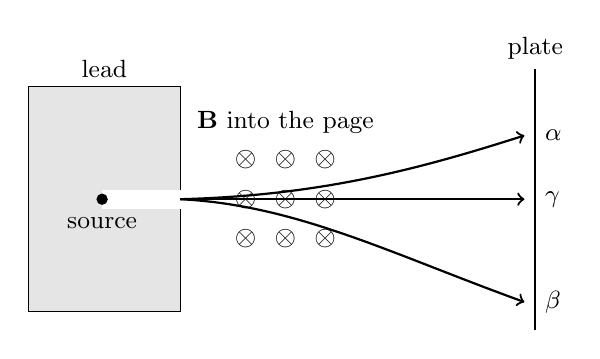
\begin{tikzpicture}[scale=0.92]
\draw[fill=gray!20] (0,-1.55) rectangle (2.1,1.55);
\draw[fill=white,draw=none] (1.02,-0.13) rectangle (2.12,0.13);
\draw[fill=black] (1.02,0) circle (0.07);
\node[below] at (1.02,-0.12) {\small source};
\node[above] at (1.05,1.55) {\small lead};
\foreach \x in {3.0,3.55,4.1}
  \foreach \y in {-0.55,0,0.55}
    \node at (\x,\y) {\(\otimes\)};
\node[above] at (3.55,0.78) {\small \(\mathbf B\) into the page};
\draw[thick] (7,-1.8) -- (7,1.8);
\node[above] at (7,1.8) {\small plate};
\draw[thick,->] (2.1,0) -- (6.85,0);
\draw[thick,->] (2.1,0) .. controls (4.0,0.05) and (5.35,0.40) .. (6.85,0.88);
\draw[thick,->] (2.1,0) .. controls (3.7,-0.08) and (5.0,-0.75) .. (6.85,-1.42);
\node[right] at (7,0.88) {\small \(\alpha\)};
\node[right] at (7,0) {\small \(\gamma\)};
\node[right] at (7,-1.42) {\small \(\beta\)};
\end{tikzpicture}
\caption{حزمة إشعاعية محزَّمة في مجال مغناطيسي مستعرض. لا ينحرف المركّب المتعادل، بينما تنحني المركّبات ذات الشحنات المتعاكسة إلى جهتين متعاكستين وبمقادير غير متساوية.}
\end{figure}

سُمّيت المكوّنات الثلاثة ألفا وبيتا وغاما. وبالمصطلحات الحديثة،
\begin{equation}
\begin{aligned}
\beta\text{-radiation} &= \text{electrons},\\
\alpha\text{-radiation} &= \text{helium nuclei},\\
\gamma\text{-radiation} &= \text{photons}.
\end{aligned}
\end{equation}
يتألف جسيم ألفا من بروتونين ونيوترونين، وهذا يفسر أن عدده الكتلي أربعة. ومن ثم، في التسلسل التقريبي للأعداد الصحيحة عند دالتون، لكان الهيليوم قد شغل الرقم أربعة: أربع وحدات نووية على مقياس الهيدروجين. أما أشعة بيتا فهي الإلكترونات سالبة الشحنة المعروفة سلفاً من تجارب الأشعة المهبطية. ولا تحمل أشعة غاما أي شحنة كهربائية.

مع مصدر منخفض الكثافة بما يكفي وكاشف قادر على تمييز كل وصول على حدة، يتحول التعريض الذي يبدو مستمرًا إلى تتابع من أحداث منفصلة: نبضة، نبضة، نبضة. ويمكن إجراء الشيء نفسه مع إشعاعات بيتا وألفا وغاما. ويعطي عدّاد غايغر الصورة الصحيحة، سواء أكان أقدم جهاز قد شُغِّل في ذلك النمط التشغيلي تحديدًا أم لا. يصل كل مكوِّن في حزم منفصلة. وتبقى أشعة غاما هي اللغز: فهي عديمة الشحنة، ومع ذلك تُكشَف حدثًا واحدًا في كل مرة. فإشعاع غاما هو ضوء ذو طاقة عالية جدًا، وقد ربط بلانك، وبخاصة أينشتاين، الضوء بالكمّات. لكن قبل مواجهة هذا الاستنتاج، لا بد من أخذ الأدلة الكلاسيكية على أن الضوء موجة على محمل الجد.

\section{الطبيعة الموجية الكلاسيكية للضوء}

في التصور الكلاسيكي، كان الضوء أوضح مثال على الاستمرارية. فهو يتكون من حقول كهربائية ومغناطيسية تنتشر على هيئة موجات متصلة. وكان نيوتن قد فضّل تصورًا جسيميًا، لكن التجارب الموجية أزاحته. إن اهتزاز شحنة يولد إشعاعًا كهرومغناطيسيًا. ويمكن لهوائي عياني أن يصدر موجات راديوية أو موجات ميكروية أو أشعة تحت الحمراء أو ضوءًا مرئيًا أو أشعة فوق بنفسجية؛ والشحنة التي تتحرك داخل الذرة هي أيضًا هوائي. ويمكن للإشعاع المنبعث أن يعرّض لوحًا فوتوغرافيًا.

تعطي فتحة واحدة أول إشارة إلى السلوك الموجي. فلو كان الضوء تيارًا من الرصاصات، لتوقعنا أن تُنتج فتحة صغيرة بقعةً ضيقةً شديدةَ الانحصار. لكن الإضاءة تنتشر بدلًا من ذلك إلى منطقة ضبابية. غير أن الانتشار وحده ليس حاسمًا، إذ يمكن تخيل جسيمات تنحرف بفعل قوى عند حافتها.

وتعطي فتحتان الاختبار الأدق. فسيعطي سيلان جسيميان مستقلان لطختين متداخلتين، ربما تكونان أشد سطوعًا حيث يتداخلان. أما الموجات فتفعل شيئًا مختلفًا. يمكن لقمة من إحدى الفتحتين أن تلتقي قمةً من الأخرى فتتعززا؛ ويمكن أيضًا لقمة أن تلتقي قاعًا فيُلغي أحدهما الآخر. ولذلك تُظهر الشاشة أشرطةً مضيئةً ومظلمةً بالتناوب، بما في ذلك مواضع مظلمة كانت أيٌّ من الفتحتين وحدها ستضيئها.\footnote{يعيد الشكل التخطيطي بناء مخططي الفتحة والتداخل اللذين جرى تطويرهما في فيديو المحاضرة بين 00:25:00 و00:29:49.}

\begin{figure}[h]
\centering
\resizebox{\linewidth}{!}{%
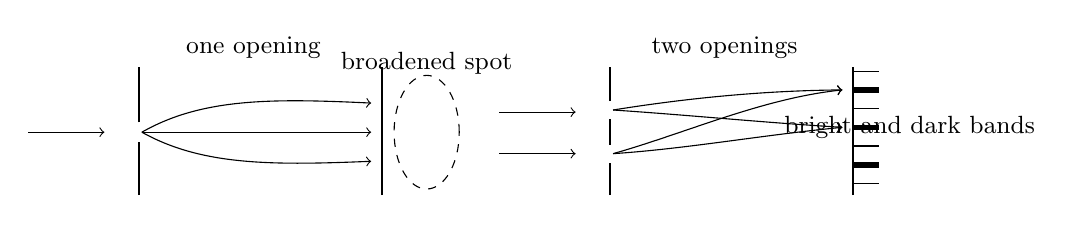
\begin{tikzpicture}[scale=0.88]
\begin{scope}
\draw[->] (-0.3,1.06) -- (0.8,1.06);
\draw[thick] (1.3,0.15) -- (1.3,0.92);
\draw[thick] (1.3,1.20) -- (1.3,2.0);
\draw[thick] (4.8,0.15) -- (4.8,2.0);
\draw[->] (1.34,1.06) .. controls (2.2,1.55) and (3.2,1.55) .. (4.65,1.48);
\draw[->] (1.34,1.06) -- (4.65,1.06);
\draw[->] (1.34,1.06) .. controls (2.2,0.58) and (3.2,0.58) .. (4.65,0.64);
\draw[dashed] (5.45,1.06) ellipse (0.47 and 0.82);
\node at (2.95,2.28) {\small one opening};
\node at (5.45,2.05) {\small broadened spot};
\end{scope}
\begin{scope}[xshift=6.8cm]
\draw[->] (-0.3,1.35) -- (0.8,1.35);
\draw[->] (-0.3,0.75) -- (0.8,0.75);
\draw[thick] (1.3,0.15) -- (1.3,0.62);
\draw[thick] (1.3,0.88) -- (1.3,1.25);
\draw[thick] (1.3,1.51) -- (1.3,2.0);
\draw[thick] (4.8,0.15) -- (4.8,2.0);
\draw[thin] (4.8,0.32) -- (5.18,0.32);
\draw[line width=2pt] (4.8,0.59) -- (5.18,0.59);
\draw[thin] (4.8,0.86) -- (5.18,0.86);
\draw[line width=2pt] (4.8,1.13) -- (5.18,1.13);
\draw[thin] (4.8,1.40) -- (5.18,1.40);
\draw[line width=2pt] (4.8,1.67) -- (5.18,1.67);
\draw[thin] (4.8,1.94) -- (5.18,1.94);
\draw[->] (1.34,0.75) .. controls (2.4,0.82) and (3.5,1.02) .. (4.65,1.13);
\draw[->] (1.34,1.38) .. controls (2.4,1.31) and (3.5,1.20) .. (4.65,1.13);
\draw[->] (1.34,0.75) .. controls (2.4,1.05) and (3.5,1.55) .. (4.65,1.67);
\draw[->] (1.34,1.38) .. controls (2.4,1.55) and (3.5,1.66) .. (4.65,1.67);
\node at (2.95,2.28) {\small two openings};
\node at (5.62,1.13) {\small bright and dark bands};
\end{scope}
\end{tikzpicture}
}
\caption{تُنتِج فتحة واحدة صورةً متسعة، بينما تُنتِج فتحتان تداخلاً بنّاءً وهدّامًا بالتناوب.}
\end{figure}

يسهل تخيّل الأثر نفسه في الماء. حرّك إصبعين على سطحه: تنتشر الموجات الدائرية، وتتَعزَّز في بعض المواضع، وتُلغي بعضها بعضًا في مواضع أخرى. إن التداخل، لا مجرد الانتشار، هو العلامة الحاسمة على السلوك الموجي.

والتسلسل التاريخي، مرة أخرى، ليس بسيطًا. ففي هذا العرض التخطيطي يُقدَّم Huygens قبل Newton بوصفه من أنصار انتشار الموجات؛ ويُربَط Thomas Young ببرهان التداخل؛ كما أن بعض تجارب Newton البصرية نفسها تقبل تفسيرًا قائمًا على تداخل الموجات، رغم أنه كان يفضّل الجسيمات. وقد أثبتت تجارب التداخل اللاحقة الطبيعة الموجية للضوء بما لا يدع مجالًا لشك معقول.

ثم حدّد Maxwell ما الذي يتذبذب. فإذا انتشرت موجة ضوئية على طول محور، فإن مجالها الكهربائي يكون مستعرضًا بالنسبة إلى ذلك المحور. ويكون مجالها المغناطيسي مستعرضًا أيضًا ومتعامدًا على المجال الكهربائي. وينتقل النمط بأكمله بسرعة الضوء.\footnote{يعيد هذا المخطط بناء رسم الموجة الكهرومغناطيسية المرسوم في فيديو المحاضرة عند 00:31:08.}

\begin{figure}[h]
\centering
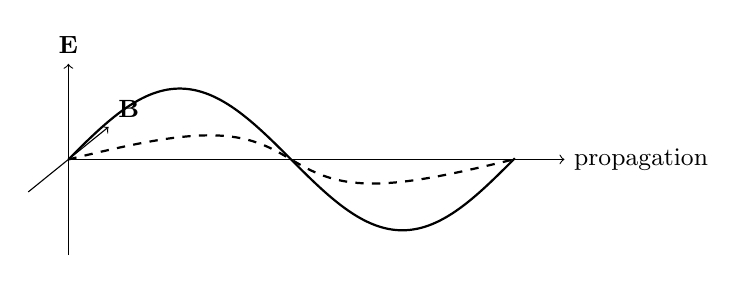
\begin{tikzpicture}[
  scale=0.9,
  x={(1cm,0cm)},
  y={(0cm,1cm)},
  z={(0.42cm,0.34cm)}
]
\draw[->] (0,0,0) -- (7,0,0) node[right] {\small propagation};
\draw[->] (0,-1.35,0) -- (0,1.35,0) node[above] {\small \(\mathbf E\)};
\draw[->] (0,0,-1.35) -- (0,0,1.35) node[above right] {\small \(\mathbf B\)};
\draw[thick,smooth,variable=\x,domain=0:6.3,samples=100]
  plot ({\x},{sin(\x r)},0);
\draw[thick,dashed,smooth,variable=\x,domain=0:6.3,samples=100]
  plot ({\x},0,{sin(\x r)});
\end{tikzpicture}
\caption{في موجة كهرومغناطيسية، يكون المجالان الكهربائي والمغناطيسي متعامدَين أحدهما على الآخر، وكلاهما مستعرض بالنسبة إلى اتجاه الانتشار.}
\end{figure}

يتذبذب الضوء المرئي العادي بسرعة أكبر بكثير من أن يمكن تتبّع الحقول المتناوبة مباشرةً. وفي موجة راديوية طويلة جدًا، يكون التذبذب أبطأ على نحو مناظر. وفي كلتا الحالتين تؤدي هندسة الموجة المستعرضة نفسها إلى التداخل.

\section{الطول الموجي، والزمن الدوري، والتردد}

الطول الموجي \(\lambda\) هو مسافة مكانية: ابدأ من نقطة في الاهتزاز وتحرك على طول الموجة حتى يتكرر الطور نفسه بعد دورة كاملة. ويُقاس بالأمتار أو بالسنتيمترات أو بأي وحدة طول أخرى.

والآن ابقَ عند موضع واحد بينما تمر الموجة. فالزمن اللازم لدورة كاملة واحدة هو الزمن الدوري \(T\). للضوء المرئي زمن دوري قصير جدًا، تقريبًا من رتبة \(10^{-15}\,\mathrm{s}\)؛ فالطول الموجي الأطول يقابله زمن دوري أطول، والأقصر يقابله زمن دوري أقصر.

خلال زمن دوري واحد، تتقدم الموجة بمقدار طول موجي واحد، لذا فإن موجة سرعتها \(v\) تخضع للعلاقة
\begin{equation}
v=\frac{\lambda}{T}.
\end{equation}
وللموجات المائية والصوتية سرعات انتشارها الخاصة. أما بالنسبة إلى الضوء،
\begin{equation}
c=\frac{\lambda}{T}.
\end{equation}
والتردد \(f\) هو عدد الدورات في وحدة الزمن:
\begin{equation}
f=\frac{1}{T}.
\end{equation}
ومن ثم
\begin{equation}
\lambda f=c.
\end{equation}
ويكفي معرفة الطول الموجي أو التردد لتحديد الآخر.

\begin{figure}[h]
\centering
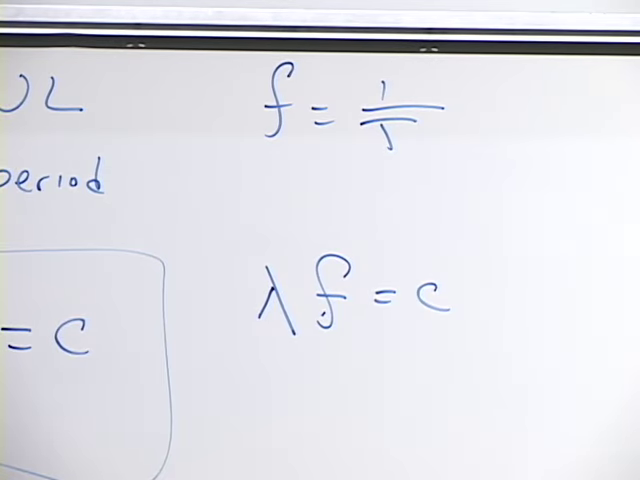
\includegraphics[width=0.68\textwidth]{lecture_01_figure_03.png}
\caption{لموجة ضوئية، \(f=1/T\) و\(\lambda f=c\).}
\lectureframe{00:36:24}
\end{figure}

غالبًا ما يقيس الفيزيائيون معدل الاهتزاز بالراديان في الثانية بدلًا من الدورات الكاملة في الثانية. تخيَّل حركة منتظمة حول دائرة. إذا أكملت النقطة \(f\) دورةً في كل ثانية، وكانت كل دورة تحتوي على \(2\pi\) راديان، فإن ترددها الزاوي هو
\begin{equation}
\omega=2\pi f,
\qquad
\frac{\omega}{2\pi}=f.
\end{equation}
وفي الوقت الحالي هذا مجرد تعريف؛ أما السؤال العملي عما إذا كان يقلل عدد عوامل \(2\pi\) فسيعود لاحقًا.

إن الجمع بين \(f=c/\lambda\) و\(\omega=2\pi f\) يعطي
\begin{equation}
\omega=\frac{2\pi c}{\lambda},
\qquad
\omega\lambda=2\pi c.
\end{equation}
أما لنوع آخر من الموجات، فيُستبدل \(c\) بسرعة انتشار تلك الموجة.

\begin{figure}[h]
\centering
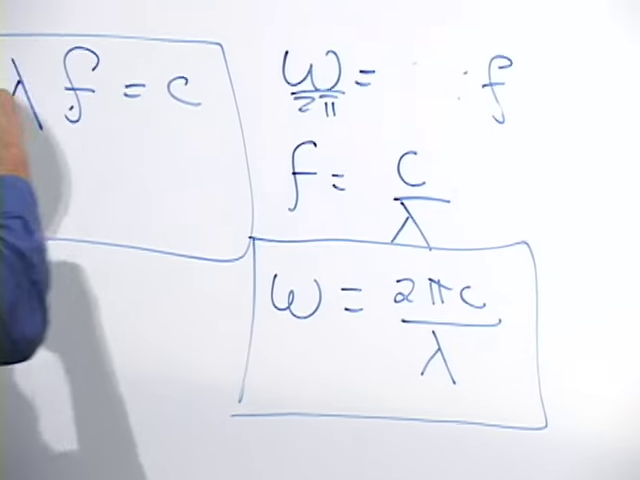
\includegraphics[width=0.68\textwidth]{lecture_01_figure_04.png}
\caption{مع \(\omega=2\pi f\)، تحقق موجة ضوئية \(\omega=2\pi c/\lambda\).}
\lectureframe{00:39:10}
\end{figure}

يشكل الإشعاع الكهرومغناطيسي طيفًا متصلًا. ومرتبةً من الأطول طولًا موجيًا إلى الأقصر، تكون الأسماء المتعارف عليها هي
\begin{equation}
\begin{aligned}
\text{radio}
&\longrightarrow \text{microwave}
\longrightarrow \text{infrared}
\longrightarrow \text{visible}\\
&\longrightarrow \text{ultraviolet}
\longrightarrow \text{X ray}
\longrightarrow \text{gamma ray}.
\end{aligned}
\end{equation}
ولا يشغل الضوء المرئي إلا مجالًا ضيقًا. والحدود بين المناطق المسماة اصطلاحية، لذلك لا حاجة هنا إلى أطوال موجية فاصلة دقيقة. قد تكون الموجات الراديوية طويلة للغاية؛ أما إشعاع غاما فهو الطرف القصير جدًا في الطول الموجي من الطيف الكهرومغناطيسي. وهنا تتضح الصعوبة بحدة: فإشعاع غاما، وفقًا للوصف الكلاسيكي، موجة حقلية متصلة، ومع ذلك يُكتشف على هيئة ومضات منفصلة.

\section{وصولات منفصلة واحتمالات الموجة}

قادت الخواص الثرموديناميكية للإشعاع بلانك وآينشتاين إلى استنتاج أن الضوء يجب أن يُعامل في وحدات منفصلة. وتجربة متخيلة تجعل هذه النقطة جلية، لكنها لا تزعم أنها المسار التاريخي الفعلي إلى الاكتشاف.

سلِّط حزمة على شاشة. عند شدة عادية، تُحدث بقعة مضيئة تبدو متصلة. ضع مُضعِّفًا معتمًا جزئيًا في الحزمة: فتصبح البقعة أخفت. زِد الإضعاف مرارًا فيصل ضوء أقل في وحدة الزمن. وفي النهاية يتغير المظهر. فبدلًا من بقعة خافتة تبدو متصلة، يسجل الكاشف أحداثًا منفصلة.\footnote{يعيد الرسم التخطيطي بناء تجربة الإضعاف كما جرى عرضها في فيديو المحاضرة بين 00:42:32 و00:45:42.}

\begin{figure}[h]
\centering
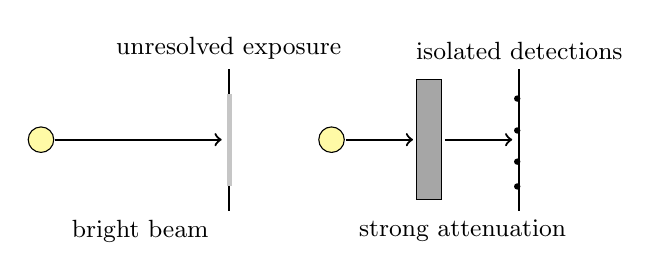
\begin{tikzpicture}[scale=0.9]
\begin{scope}
\draw[fill=yellow!35] (0,0) circle (0.18);
\draw[->,thick] (0.2,0) -- (2.55,0);
\draw[thick] (2.65,-1.0) -- (2.65,1.0);
\node[below] at (1.4,-1.0) {\small bright beam};
\end{scope}
\begin{scope}[xshift=4.1cm]
\draw[fill=yellow!35] (0,0) circle (0.18);
\draw[->,thick] (0.2,0) -- (1.15,0);
\draw[fill=gray!70] (1.2,-0.85) rectangle (1.55,0.85);
\draw[->,thick] (1.6,0) -- (2.55,0);
\draw[thick] (2.65,-1.0) -- (2.65,1.0);
\node[below] at (1.85,-1.0) {\small strong attenuation};
\end{scope}
\fill[gray!45] (2.62,-0.65) rectangle (2.70,0.65);
\foreach \y in {-0.66,-0.31,0.13,0.58}
  \fill (6.72,\y) circle (0.045);
\node[above] at (2.65,1.0) {\small unresolved exposure};
\node[above] at (6.75,1.0) {\small isolated detections};
\end{tikzpicture}
\caption{يخفض الإضعاف التدريجي معدل الكشف حتى ينحلَّ تعريض يبدو متصلًا إلى أحداث فوتونية منفصلة.}
\end{figure}

إذا انتظرت مدة كافية، تراكمت تلك الأحداث لتكوِّن التوزيع المكاني نفسه للبقعة الأصلية. ولذلك كانت المنطقة المضيئة هي المجموع غير المفصول لوصولات فردية كثيرة. ويمكن إجراء هذا الاختبار عند شدة منخفضة، مع أنه لم يكن التجربة المبكرة التي حفزت في الأصل فرضية الفوتون. وقد نشأ اقتراح آينشتاين للفوتون من اعتبارات ترموديناميكية وكهروضوئية؛ وتوفر تجربة الإضعاف طريقة مباشرة على نحو خاص لتصوُّر نتيجته.

ضع الآن فتحتين في الحزمة وخفِّض الشدة حتى تصل الفوتونات واحدًا تلو الآخر. وكل عملية كشف هي ومضة موضعية. ومع ذلك، بعد عمليات كشف كثيرة، تملأ الومضات نمط تداخل، بما في ذلك أهداب مضيئة ومظلمة. الوصولات المنفصلة عشوائية، لكن توزيع احتمالاتها هو التوزيع الذي يتنبأ به النمط الموجي. لقد أصبحت الموجة الكلاسيكية موجةً تحكم الاحتمالات.

فالموجة والجسيم ليسا إذن نوعين منفصلين من الكيانات يُنسب كل منهما إلى جزء مختلف من الطبيعة. بل هما مظهران لشيء كمومي واحد. ولا يمكن وصف الضوء وصفًا كافيًا على أنه موجة فقط أو جسيم فقط.

أما الإلكترونات فتعكس المفاجأة الأصلية. فقد كان يُسلَّم بأن الإلكترونات جسيمات، وهي تصل إلى كاشف واحدةً تلو الأخرى، لكنها، إذا كانت الفتحات متقاربة بما يكفي، تُنشئ أيضًا نمط تداخل. وجسيمات ألفا، وهي أثقل من الإلكترونات بنحو ثمانية آلاف مرة، تخضع للمبدأ نفسه، وإن كانت التجربة أشد صعوبة. وقد لوحظ التداخل حتى مع buckyballs: جزيئات مكوَّنة من ستين ذرة كربون مرتبة تقريبًا على هيئة كرة قدم معممة. ومن المتوقع أن ينطبق المبدأ نفسه حتى على كرات البولينغ، رغم أن مثل هذه التجربة غير عملية على نحو يكاد يكون خياليًا. ويمكن المضي في المناقشة إلى تجارب مقترحة على الفيروسات أو الخلايا الحية، بوصفها أمثلة يزداد طموحها. وفهم كيف ينسجم الوصفان الموجي والجسيمي يتطلب ميكانيكا الكم؛ أما المهمة المباشرة فهي استخلاص خصائص الفوتون اللازمة لفيزياء الجسيمات.

\section{طاقة الفوتون}

الفوتونات هي العناصر المنفصلة غير القابلة للانقسام للضوء. يحمل الضوء طاقة---فضوء الشمس يسخِّن جسمًا ماصًّا---لذا لا بد أن يحمل كل فوتون طاقة. للموجة الأحادية اللون طول موجي وتردد زاوي محددان، وتكون طاقة كل فوتون فيها:
\begin{equation}
E_\gamma=\hbar\omega.
\end{equation}
ومن المضلل أن نحاول تصور موجة متصلة على أنها تجمّع ميكانيكي صغير من النقاط. وما هو مؤكد هو هذا التركيب التجريبي: تحدث عمليات كشف موضعية وفق توزيع تحكمه الموجة، وتصل الطاقة في وحدات غير قابلة للانقسام.

وبما أن
\begin{equation}
\omega=\frac{2\pi c}{\lambda},
\end{equation}
فإن الطول الموجي الأقصر يعني ترددًا زاويًا أكبر، ومن ثم طاقة أكبر في كل فوتون:
\begin{equation}
\lambda\downarrow
\quad\Longrightarrow\quad
\omega\uparrow
\quad\Longrightarrow\quad
E_\gamma\uparrow.
\end{equation}
طاقة الفوتون الراديوي الواحد صغيرة جدًا. ومع ذلك، يمكن لحزمة راديوية أن تحمل طاقة كلية هائلة لأنها تحتوي على عدد كبير جدًا من الفوتونات. ولنبضة أحادية اللون تحتوي على \(n\) فوتونًا،
\begin{equation}
E_{\text{pulse}}=n\hbar\omega,
\qquad
n=0,1,2,\ldots.
\end{equation}
قد يكون المجموع كبيرًا، لكنه يظل مضاعفًا صحيحًا لطاقة الفوتون الواحد.

تشير هذه العلاقة إلى السؤال العملي الذي سيحكم بقية المناقشة. لماذا يجب بناء آلات أكبر فأكبر لرؤية أشياء أصغر فأصغر؟ ولماذا لا نستخدم آلة صغيرة لشيء صغير؟ النصف الأول من الجواب حاضر بالفعل: فتمييز بنية أصغر فأصغر يتطلب طولًا موجيًا أقصر، والكم ذو الطول الموجي الأقصر يحمل طاقة أكبر.

\section{طاقة السكون والكتلة اللامتغيرة}

تجمع فيزياء الجسيمات بين ميكانيكا الكم والنسبية. وتوفّر علاقة الفوتون \(E_\gamma=\hbar\omega\) الجانب الكمّي؛ أمّا الحقيقة الأولية المناظرة من النسبية فهي
\begin{equation}
E_{\mathrm{rest}}=mc^2.
\end{equation}
وهذا التقييد مهم. فقد ميّزت العروض الأقدم بين \emph{كتلة السكون} وبين \emph{الكتلة المتحركة} المعتمدة على السرعة. ويستعمل الاصطلاح الحديث \emph{الكتلة} للدلالة على الكتلة الثابتة لجسم ما. فالحركة تغيّر طاقته لا كتلته. ولكل إلكترون الكتلة نفسها مهما كانت حالته الحركية، في حين تزداد طاقة الإلكترون كلما عُجِّل. ومن ثم فإن \(E=mc^2\)، في هذه الصيغة، هي طاقة جسم ذي كتلة في إطار يكون فيه الجسم ككل ساكنًا.

ليس من الضروري أن يكون الجسم ساكنًا داخليًا. يمكن لصندوق من الغاز أن يبقى ساكنًا على ميزان بينما تتحرك جزيئاته بسرعة في جميع الاتجاهات. وطاقة تلك الحركات الداخلية جزء من طاقة السكون للصندوق بأكمله. ابدأ بصندوق بارد، وقِس كتلته، ثم أضف طاقة حرارية مع إبقاء الصندوق نفسه ساكنًا. فتتغير كتلته الساكنة بمقدار
\begin{equation}
\Delta m=\frac{\Delta E_{\mathrm{internal}}}{c^2}.
\end{equation}
ويزداد وزنه وقصوره الذاتي مع كتلته. وبالنسبة إلى صندوق عادي، حتى بعد ارتفاع كبير في درجة الحرارة، يكون الأثر أصغر بكثير من أن يُلاحظ على ميزان عادي؛ وصِغَر الأثر لا يغيّر المبدأ.

ويأتي مثال أوضح باستخدام إلكترون وبوزيترون. فلهما كتلتان متساويتان تمامًا وشحنتان كهربائيتان متعاكستان. وإذا كانا في البداية ساكنين ثم أفنيا بعضهما، حملت الفوتونات الطاقة بعيدًا:
\begin{equation}
e^-+e^+\longrightarrow \text{photons}.
\end{equation}
والطاقة الابتدائية هي
\begin{equation}
E_{\mathrm{initial}}=2m_e c^2,
\end{equation}
ولا يمكن لتلك الطاقة أن تختفي. ولا يعطي زوج واحد إلا مقدارًا ضئيلًا جدًا، لذا يلزم عدد هائل من الأزواج لتسخين حتى فنجان من القهوة، لكن أحداث الإفناء الفردية تُظهر التحول مباشرةً.

لذلك، بالنسبة إلى جسم ساكن، تكون الكتلة والطاقة الكمية الفيزيائية نفسها مُعبَّرًا عنها بوحدتين مختلفتين. والعامل \(c^2\) هو عامل التحويل بين وحدات الكتلة والطاقة المألوفة، تمامًا كما يحوّل عامل عددي الأمتار إلى سنتيمترات.

\begin{classroomqa}
\lecturetimestamp{01:04:39}
\audiencequestion{هل يتطلب تحويل الكتلة إلى طاقة منطلقة آليةً ما؟}
\lecturerresponse{نعم، يلزم وجود آلية فيزيائية، لكن قوانين الانحفاظ تقيّد نتيجتها سلفًا. فحتى قبل وصف آلية الإفناء المجهرية، لا بد أن تعاود الظهور في مكان ما الطاقة الابتدائية للإلكترون--البوزيترون. لذلك يمكن لانحفاظ الطاقة أن يحدد جزءًا مهمًا من الجواب من غير عرض تفصيلي للتفاعل.}
\end{classroomqa}

\section{الأبعاد واختيار الوحدات}

في وحدات النظام الدولي، تكون سرعة الضوء عددًا كبيرًا جدًا ويكون ثابت بلانك عددًا صغيرًا جدًا. ويُوحي بصِغَر هذا الأخير أصلًا علاقة الفوتون: فالتردد الزاوي للضوء المرئي هائل، في حين أن طاقة فوتون واحد ضئيلة، لذا تتطلب \(E_\gamma=\hbar\omega\) قيمة عددية صغيرة لـ\(\hbar\) في هذه الوحدات. وعلى مستوى رتبة المقدار،
\begin{equation}
c\sim 10^8\ \mathrm{m\,s^{-1}},
\qquad
\hbar\sim 10^{-34}\ \mathrm{J\,s}.
\end{equation}
\editorialnote{لم يُحتفَظ إلا برتب المقدار المذكورة في المحاضرة لأن الأرقام الأخيرة على اللوح غير واضحة.}
والوحدات أساسية: فليس أيٌّ من الثابتين مجرد عدد عشري صرف. وبما أن للطاقة الأبعاد
\begin{equation}
[E]=M L^2 T^{-2},
\end{equation}
وأن \(E_\gamma=\hbar\omega\) مع \([\omega]=T^{-1}\)، فإن ثابت بلانك له الأبعاد
\begin{equation}
[\hbar]=[E]T=M L^2 T^{-1}.
\end{equation}

إن وصف \(c\) بالكِبَر و\(\hbar\) بالصِّغَر يفترض سلفًا اختيارًا للوحدات. فقياس السرعة بالأقدام في الساعة يعطي قيمة عددية لـ\(c\) تختلف عن قياسها بالأمتار في الثانية. وبوحدات السنوات الضوئية لكل سنة، أو الثواني الضوئية لكل ثانية، تكون سرعة الضوء ببساطة واحدًا. وبالمثل، يمكن لاختيار مناسب ومنسق لوحدات الكتلة والطول والزمن أن يجعل \(\hbar=1\).

أنظمة الوحدات المألوفة أعراف متوارثة، لا خصائص مميزة للطبيعة. فالميل الواحد يضم 5280 قدمًا، ووحدة stone تضم أربعة عشر رطلًا، وتُقاس الخيول بوحدة اليد، وقد تُقاس القدرة بالقدرة الحصانية. والوحدات المترية أكثر انتظامًا، لكن مقاييسها تظل اختيارات بشرية. وليس في الفيزياء الأساسية ما يميّز المتر أو الثانية أو الكيلوغرام.

يتيح الطول والزمن والكتلة ثلاثة اختيارات أساسية مستقلة للوحدات:
\begin{equation}
L,\qquad T,\qquad M.
\end{equation}
ويمكن بناء سائر الوحدات الميكانيكية منها. وتعتمد الاختيارات المفيدة على المسألة. فكتلة شمسية مريحة في الفيزياء الفلكية؛ وقد تكون كتلة البروتون مريحة في الفيزياء النووية؛ كما تجعل السنوات الضوئية والسنوات الصيغ الفلكية النسبية أكثر إيجازًا. ومع وجود ثلاثة اختيارات مستقلة، يمكن إسناد قيم عددية مناسبة إلى ثلاثة ثوابت ذات أبعاد مستقلة. وليس من الضروري أن تتخذ الفيزياء الفلكية والفيزياء الذرية وفيزياء الجسيمات الاختيارات نفسها.

في فيزياء الجسيمات، هناك اصطلاحان مفيدان على نحو خاص هما
\begin{equation}
c=1,
\qquad
\hbar=1.
\end{equation}
ولا توجد كتلة لجسيم تتميز على نحو مماثل بالنسبة إلى الوحدة المتبقية. ويمكن للمرء أن يعلن أن كتلة البروتون، أو كتلة بوزون هيغز، أو كتلة الميون تساوي واحدًا، لكن ذلك لن يكون إلا تفضيلًا لعنصر واحد من مجموعة كبيرة.

فلماذا نختار \(c\) و\(\hbar\) إذن؟ قد يكون الجواب الأول أنهما يظهران في معادلات كثيرة. لكن كثرة الظهور لا تكفي: فكتلة البروتون تظهر أيضًا في معادلات كثيرة، وكذلك حجم البروتون. وما يميز \(c\) و\(\hbar\) هو كونيتهما.

الثابتان \(c\) و\(\hbar\) مختلفان. فالسرعة \(c\) تقيّد كل جسم فيزيائي: إذ يمكن للأجسام ذات الكتلة أن تقترب منها، ولكن لا يمكن تسريعها لتتجاوزها. ويقيّد ثابت بلانك كل جسم كمومي من خلال علاقة الارتياب على مستوى رتبة المقدار
\begin{equation}
\Delta x\,\Delta p\gtrsim\hbar.
\end{equation}
ولا تخص أيٌّ من العبارتين نوعًا بعينه من الجسيمات. وهذه الكونية هي ما يجعل \(c=1\) و\(\hbar=1\) اصطلاحين طبيعيين.

ولا يوفّر البروتون مقياسًا كونيًا مماثلًا. فهو مجرد جسم واحد بين أشياء كثيرة. وجعل كتلة البروتون مساوية لواحد لا يتمتع بمكانة أكثر أساسية من جعل كتلة ذرة روبيديوم مساوية لواحد؛ ويعرض الإلكترون وبوزون هيغز والميون الصعوبة نفسها.

وتوحي الشحنة الكهربائية بكمية كونية أخرى، لكن بعد جعل \(c\) و\(\hbar\) مساويين لواحد، يصبح الاقتران الكهرومغناطيسي ذو الدلالة الفيزيائية بلا أبعاد. ويمكن لتغيير الوحدات أن ينقل الثوابت ذات الأبعاد داخل صيغة كهرومغناطيسية؛ لكنه لا يستطيع تغيير اقتران حقيقي بلا أبعاد.

وتوفّر الجاذبية ثابتًا كونيًا ذا أبعاد. ففي الصيغة النيوتونية، يكون مقدار القوة بين كتلتين
\begin{equation}
F=G\frac{m_1m_2}{r^2}.
\end{equation}
وكل كتلة تتفاعل ثقاليًا، في حين إن الأجسام المتعادلة كهربائيًا ليست مضطرة إلى المشاركة في قوة كهربائية. ومن ثم يملك \(G\) الكونية المطلوبة. ومع ذلك، فهو تطبيع عملي رديء لفيزياء الجسيمات العادية، لأن قوى الجاذبية بين الجسيمات الأولية المعروفة مهملة في الحسابات موضع النقاش.

\begin{classroomqa}
\lecturetimestamp{01:20:34}
\audiencequestion{هل يصح ببساطة استبعاد \(G\)؟ فعند طاقات عالية جدًا قد لا تطيع الجسيمات الأولية الجاذبية الكلاسيكية على النحو المفترض.}
\lecturerresponse{تستجيب الجسيمات المفردة فعلًا لحقل الجاذبية الأرضي: فالجسيم الواحد يسقط في ذلك الحقل. ولم يُقَس الأثر الثقالي لجسيم أولي واحد على آخر قياسًا مباشرًا، لذا يمكن التشكيك في افتراض الكونية عند ذلك المستوى. والسبب المباشر لترك \(G\) خارجًا هو سبب عملي لا مطلق: فالجاذبية تسهم إسهامًا مهملًا في تجارب فيزياء الجسيمات العادية ومعادلاتها.}
\end{classroomqa}

\begin{classroomqa}
\lecturetimestamp{01:22:01}
\audiencequestion{هل يمكن استعمال التفاعل الكهربائي بوصفه الاصطلاح الثالث لتحديد الوحدات بدلًا من الجاذبية؟}
\lecturerresponse{نعم. يمكن اختيار وحدات كهرومغناطيسية تُطبَّع فيها الشحنة الكهربائية، أو الثابت الذي يظهر في قانون كولوم. وتُستعمل مثل هذه الاصطلاحات. فالإلكترونات تتنافر بدلًا من أن تتجاذب، لكن تلك الإشارة لا تعوق الاختيار. إنه ببساطة ليس الاصطلاح المعتمد هنا.}
\end{classroomqa}

\begin{classroomqa}
\lecturetimestamp{01:23:06}
\audiencequestion{بمجرد جعل \(c\) و\(\hbar\) مساويين لواحد، هل تصبح الشحنة الكهربائية بلا أبعاد؟}
\lecturerresponse{نعم. فهناك مقدار بلا أبعاد يرتبط بمربع الشحنة الكهربائية يساوي تقريبًا \(1/137\). ويمكن إرجاء الاصطلاح الدقيق ومعنى ذلك العدد؛ والنقطة هنا هي أنه بلا أبعاد.}
\end{classroomqa}

\begin{classroomqa}
\lecturetimestamp{01:23:37}
\audiencequestion{هل يمكن اختيار ثابت كولوم بوصفه الثابت الثالث الذي يُجعل مساويًا لواحد؟}
\lecturerresponse{يمكن امتصاصه في اصطلاح الوحدات الكهرومغناطيسية. ولا يمكن لهذا الاختيار أن يحوّل الاقتران اللابُعدي \(1/137\) إلى واحد، لأن تغيير الوحدات لا يمكن أن يغيّر عددًا بلا أبعاد. ولا يُدَّعى هنا أي نفع خاص من اعتماد ذلك الاصطلاح.}
\end{classroomqa}

\section{معادلات الوحدات الطبيعية والأطر المرجعية}

مع \(c=1\)، تصبح علاقة طاقة السكون لجسم ذي كتلة على الصورة
\begin{equation}
E_{\mathrm{rest}}=m.
\end{equation}
ومع \(\hbar=1\)، تصبح علاقة الفوتون على الصورة
\begin{equation}
E_\gamma=\omega.
\end{equation}
ويمكن إعادة إدخال الثابتين كلما احتيج إلى مقادير عددية بوحدات مألوفة.

\begin{figure}[h]
\centering
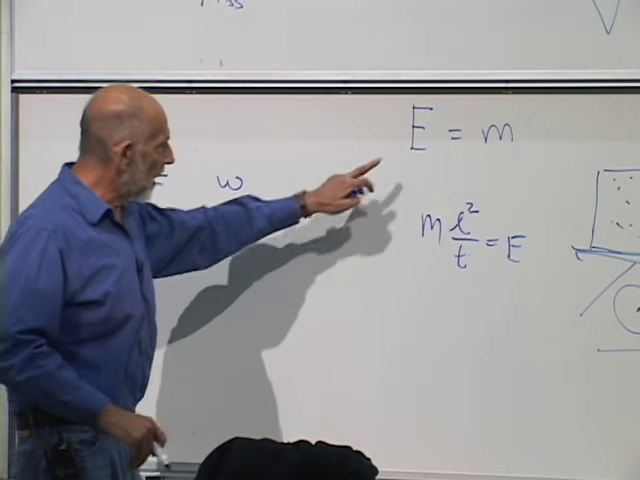
\includegraphics[width=0.72\textwidth]{lecture_01_figure_05.png}
\caption{في وحدات يكون فيها \(c=1\)، تكون طاقة السكون لجسم ذي كتلة في حالة سكون هي \(E=m\).}
\lectureframe{01:25:40}
\end{figure}

تبدو هذه الصيغ متشابهة، لكنها تعني أشياء مختلفة. في \(E_{\mathrm{rest}}=m\)، تمثل \(E\) طاقة السكون لجسم ذي كتلة. والفوتون عديم الكتلة ولا يمكن إحضاره إلى السكون، لذا فإن طاقته ليست طاقة سكون. وتعطي العلاقة \(E_\gamma=\omega\) طاقة كمٍّ متحرك عديم الكتلة.

\begin{classroomqa}
\lecturetimestamp{01:26:07}
\audiencequestion{ما معنى \emph{في حالة سكون} عندما يكون السكون دائمًا بالنسبة إلى شيء ما، والمختبر نفسه ليس في سكون مطلق؟}
\lecturerresponse{يُعرَّف السكون بالنسبة إلى إطار مختار. فإذا كان كوب ساكنًا بالنسبة إلى المختبر، فإن طاقته في إطار المختبر ذاك هي كتلته عندما \(c=1\)، من دون أي إسهام حركي كلي. أما راصد آخر يمر بجانب الكوب فيسند إليه طاقة حركية أيضًا. وبوجه عام، يسند راصدون مختلفون طاقات مختلفة إلى الجسم نفسه أو إلى الفوتون نفسه؛ فالطاقة تعتمد على الإطار المرجعي، ولا يقتضي ذلك أي ادعاء بوجود سكون مطلق.}
\end{classroomqa}

يمكن الآن إعادة النظر في اصطلاح التردد الزاوي. إن كتابة \(E_\gamma=\hbar\omega\) موجزة، لكن \(\omega=2\pi f\) أدخلت عاملًا مقداره \(2\pi\) في وقت سابق.

\begin{classroomqa}
\lecturetimestamp{01:28:13}
\audiencequestion{لماذا نستخدم التردد الزاوي \(\omega\)، المقاس بالراديان في الثانية، بدلًا من العدد الذي يبدو أبسط للدورات الكاملة في الثانية؟}
\lecturerresponse{الاختيار تاريخي جزئيًا، والإجابة الرياضية عملية أكثر منها مباشرة. والإجابة المطروحة هنا مبدئية: اكتب المعادلات ذات الصلة مرة باستعمال \(f\) ومرة باستعمال \(\omega\)، ثم انظر أي الاصطلاحين يترك عوامل أقل من \(2\pi\). ولا يمكن جعل عوامل \(2\pi\) تختفي في كل موضع. وقد اقتُرح أيضًا ارتباط محتمل بترميز الأسّ المركب، لكنه لا يُطوَّر هنا.}
\end{classroomqa}

\begin{classroomqa}
\lecturetimestamp{01:29:51}
\audiencequestion{هل يمكن تسريع جسيمين حتى يصبح تفاعلهما الثقالي المتبادل مهمًّا؟}
\lecturerresponse{من حيث المبدأ، نعم. أما عمليًا، فالمعجلات الحالية بعيدة على نحو استثنائي عن ذلك النطاق. وتعتمد الإجابة أيضًا على المقصود بكلمة جسيم: فالجسم العياني ذو الجاذبية ليس هو حالة الجسيم الأولي المقصودة هنا.}
\end{classroomqa}

\begin{classroomqa}
\lecturetimestamp{01:30:27}
\audiencequestion{ما الذي يمكن أن يكون مصدرًا للبوزيترونات؟}
\lecturerresponse{يمكن للتصادمات عالية الطاقة أن تُنتج بوزيترونات. كما تنتجها بعض العمليات النووية وبعض الاضمحلالات أيضًا.}
\end{classroomqa}

\begin{classroomqa}
\lecturetimestamp{01:30:53}
\audiencequestion{هل زمن بلانك ومسافة بلانك هما الوحدتان الطبيعيتان المستخدمتان هنا؟}
\lecturerresponse{لا. تنشأ وحدات بلانك عندما تُجعل \(G\) و\(c\) و\(\hbar\) جميعها مساويةً للواحد. ويكون طول بلانك الناتج أصغر بكثير من مقاييس الطول المعتادة في فيزياء الجسيمات، لذا فهو مقياس غير ملائم هنا. وتكون مثل هذه الوحدات طبيعية عندما تكون الجاذبية وميكانيكا الكم والنسبية كلها مهمة معًا، كما في فيزياء الثقوب السوداء أو علم الكونيات أو الجاذبية الكمومية. وعندما تكون الجاذبية مهملة، يكون جعل \(c\) و\(\hbar\) فقط مساويين للواحد أكثر فائدة.}
\end{classroomqa}

\section{الزخم والضوء والاستبانة}

المفهوم الأساسي التالي هو الزخم. الجسم الساكن لا يملك زخمًا، مع أن له طاقة سكون غير منعدمة هي \(mc^2\). وما إن يتحرك حتى يحمل، في العموم، زخمًا. ويُحفَظ الزخم في التصادم كما تُحفَظ الطاقة: فعندما يتصادم جسمان، يكون الزخم المتجهي الكلي قبل التصادم وبعده هو نفسه. وأي شيء يقيّده قانون حفظ يستحق اهتمامًا خاصًا.

الزخم كمية متجهة: فهو يشير في اتجاه الحركة. ولجسم غير نسبي،
\begin{equation}
\mathbf p=m\mathbf v.
\end{equation}
وليست هذه هي الصيغة النسبية العامة، ولا يمكن تطبيقها مباشرة على الضوء.

ومع ذلك، يحمل الضوء زخمًا كما يحمل طاقة. ويولد الضوء العادي دفعًا ضئيلًا جدًا بحيث يصعب ملاحظة زخمه، لكن نبضة ليزر شديدة يمكن أن تنقل اندفاعًا معتبرًا. فالليزر الكبير في Livermore، على سبيل المثال، يمكنه أن يدفع المادة إلى الداخل بالزخم الذي يحمله إشعاعه.

تأمل نبضة ذات توازٍ جيد بما يكفي بحيث تسير أشعتها تقريبًا على طول محور واحد. وقد يكون للحزمة الحقيقية بعض الانتشار الزاوي، بحيث تسير أجزاء منها في اتجاهات مختلفة قليلًا، لكن في الحزمة المثالية المتوازية يشير الزخم على امتداد الحزمة ويكون مقداره
\begin{equation}
p=\frac{E}{c},
\qquad\text{or equivalently}\qquad
E=cp.
\end{equation}
وتُتخذ هذه العلاقة هنا بوصفها حقيقة نسبية بدلًا من البرهنة عليها. ولا يؤكد الفحص البعدي الآتي إلا أن وحداتها تتفق مع وحدات الزخم المعتاد:
\begin{equation}
\left[\frac{E}{c}\right]
=
\frac{M L^2 T^{-2}}{L T^{-1}}
=
M L T^{-1}
=
[m v]
=
[p].
\end{equation}
ولا تُسنِد هذه المقارنة البعدية كتلة سكون إلى الضوء. فالفوتون كتلته صفر؛ وهو يحمل زخمًا لأنه يحمل طاقة ويتحرك بسرعة \(c\).

اتجاه \(\mathbf p\) هو اتجاه الانتشار. وعادةً يصعب كشف مقداره لأن \(c\) تظهر في المقام. ويمكن للحزمة أن تكشف عن طاقتها بسهولة بتسخين المادة أو تبخيرها، في حين يكون دفعها الميكانيكي أصغر بكثير. ومع شدة كافية، يمكن أن يصبح ذلك الدفع كبيرًا.

لفوتون واحد،
\begin{align}
p_\gamma
&=\frac{E_\gamma}{c}\\
&=\frac{\hbar\omega}{c}.
\end{align}
وللتعبير عن ذلك بدلالة الطول الموجي، نعود بحذر إلى علاقات الموجة. وبما أن
\begin{equation}
f\lambda=c,
\qquad
\omega=2\pi f,
\end{equation}
فالعلاقة الصحيحة هي
\begin{equation}
\omega\lambda=2\pi c,
\qquad
\omega=\frac{2\pi c}{\lambda}.
\end{equation}
ومن السهل قلب عامل \(2\pi\) إذا لم تُكتب التعريفات صراحةً. والبدء من جديد من \(f\lambda=c\) و\(f=\omega/(2\pi)\) يحسم الأمر:
\begin{equation}
\frac{\omega}{2\pi}\lambda=c
\quad\Longrightarrow\quad
\omega\lambda=2\pi c.
\end{equation}
ويعطي التعويض الآن
\begin{align}
p_\gamma
&=\frac{\hbar}{c}\frac{2\pi c}{\lambda}\\
&=\frac{2\pi\hbar}{\lambda}\\
&=\frac{h}{\lambda}.
\end{align}

\begin{classroomqa}
\lecturetimestamp{01:42:38}
\audiencequestion{هل \(2\pi\hbar\) يساوي \(h\)؟}
\lecturerresponse{نعم. فبحسب التعريف \(h=2\pi\hbar\)، لذا فإن \(p_\gamma=2\pi\hbar/\lambda\) هو نفسه \(p_\gamma=h/\lambda\). وتظهر عوامل \(2\pi\) من جديد في موضع ما أيًّا كان اصطلاح التردد المختار.}
\end{classroomqa}

كلما قصر الطول الموجي كبر زخم الفوتون. لفوتون الراديو طول موجي طويل جدًا وزخم ضئيل جدًا. أما فوتون أشعة غاما فطوله الموجي قصير جدًا ودفعتُه أكبر بكثير. ولا يزال فوتون واحد لا يعطي إلا اندفاعًا عيانيًا صغيرًا، لكن زخمه أكبر بكثير من زخم فوتون راديو. وطاقته أكبر أيضًا، لأن \(E_\gamma=cp_\gamma\).

تفسر هذه العلاقة لماذا تتطلب الأجسام الأصغر آلات أكبر. فالصورة الملتقطة بأطوال موجية أطول بكثير من رأس الإنسان لا يمكن أن تُظهر إلا غشاوة. ولتمييز ملامح الوجه، يجب أن يكون الطول الموجي أقصر من الرأس. ولتمييز شعرة واحدة، يجب أن يكون مماثلًا لسماكة الشعرة أو أصغر منها. ولتمييز بنية ذرة، يجب ألا يزيد الطول الموجي للمسبار على الذرة:
\begin{equation}
\lambda_{\mathrm{probe}}\lesssim
\text{size of the structure to be resolved}.
\end{equation}
ولذلك تتطلب البنى الأصغر أطوالًا موجية أقصر، وتتطلب الأطوال الموجية الأقصر زخمًا وطاقة أكبر. ولا يلزم أن يكون المسبار فوتونًا؛ فالجسيمات العالية الطاقة من أنواع أخرى تخضع للصلة الكمومية نفسها بين الطول الموجي والزخم. ويتطلب إنتاجها معجلات تنقل إلى كل جسيم طاقة أكبر فأكبر. وتكفي العلاقتان \(p_\gamma=h/\lambda\) و\(E_\gamma=\hbar\omega\) لإقامة هذه الحجة: فزيادة طاقة المسبار تزيد زخمه وتقصّر طوله الموجي.

كان هذا هو النمط المتكرر في فيزياء الجسيمات طوال نحو قرن: طاقة أعلى، وزخم أكبر، وطول موجي أقصر، واستبانة مكانية أدق.

\begin{classroomqa}
\lecturetimestamp{01:46:57}
\audiencequestion{هل يوجد حد أدنى نظري للطول الموجي؟}
\lecturerresponse{ربما. يُتوقع شيء جديد قرب طول بلانك، لكن الإجابة غير جازمة. وإذا كان حدّ الاستبانة المكانية يقع هناك، فإن ذلك المقياس لا يزال أصغر بنحو سبعة عشر رتبة مقدار من المسافات التي يجري سبرها في LHC، لذا تبقى التجارب الحالية بعيدة عنه على نحو هائل.}
\end{classroomqa}

وتشير سلسلة الاستدلال نفسها إلى صلة تقريبية بين مقياس المعجّل والمقياس الذي يستطيع تمييزه.

\begin{classroomqa}
\lecturetimestamp{01:48:02}
\audiencequestion{هل يرتبط الطول الموجي، أو الحجم الذي يجري تمييزه، تقريبًا بعلاقة عكسية مع حجم المعجّل؟}
\lecturerresponse{تقريبًا، نعم، بشرط أن تبقى الحقول الكهربائية العظمى التي تسرّع الجسيمات، والحقول المغناطيسية المستخدمة في توجيهها، ثابتة ضمن ما يتيحه الجهاز المتاح. وتدرج التسريع هو كسب في الطاقة لكل وحدة طول. وفي معجّل خطي طوله \(L\) وتدرج ثابت تقريبًا مقداره \(\mathcal G\)،
\[
E_{\mathrm{beam}}\sim \mathcal G L.
\]
وعند الطاقات الفائقة النسبية يرتبط الطول الموجي القابل للتمييز عكسيًا بالطاقة، لذا فإن زيادة طول المعجّل الخطي تحسّن الاستبانة تقريبًا بالعامل المعكوس. وهذا مجرد تحجيم استدلالي، لا قانونًا دقيقًا. وتتيح الآلات الدائرية اجتياز الجهاز نفسه مرارًا، لكن الشحنات المسرّعة تشع أثناء انحنائها وتفقد طاقة.}
\end{classroomqa}

\begin{classroomqa}
\lecturetimestamp{01:49:47}
\audiencequestion{ما كِبَر المعجّل الذي سيلزم لبلوغ طول بلانك؟}
\lecturerresponse{وفق هذا التحجيم التقريبي، سيلزم أن يكون أطول بنحو سبعة عشر رتبة مقدار من معجّل CERN. وهذا ليس بحجم الكون، لكنه يقع تقريبًا على مقياس مجري.}
\end{classroomqa}

\begin{classroomqa}
\lecturetimestamp{01:50:09}
\audiencequestion{كيف تُقارَن طاقات الأشعة الكونية الأعلى طاقةً بطاقات المصادمات؟}
\lecturerresponse{يمكن للشعاع الكوني الواحد أن يحمل طاقة مخبرية أكبر بكثير. ولأجل المقارنة العددية، خذ شعاعًا كونيًا متطرفًا ذا طاقة مخبرية من رتبة \(10^{21}\,\mathrm{eV}=10^{12}\,\mathrm{GeV}\). لكن الشعاع الكوني يصطدم بهدف ساكن في المختبر، في حين يُدخل المصادم حزمتين عاليتي الطاقة في تصادم جبهي. والأهم من ذلك أن التجارب المفيدة تتطلب فيضًا: عددًا كبيرًا من الجسيمات وكثيرًا من التصادمات المضبوطة جيدًا. فقد يُخطئ شعاع كوني منفرد الهدفَ المعني، أو يُنتج حدثًا لا يمكن استنتاج الكثير منه. وقدَّر تقديرٌ بالمكافئ النفطي، مقصودٌ به المبالغة، الإمدادَ اللازم لتشغيل مُسرِّع مجرّي مفيد بنحو مئة تريليون برميل من النفط في الثانية. والغرض منه هو إظهار أن إحصاءات التصادمات الكافية ستكون على الأقل عقبةً جسيمة بقدر طول المُسرِّع.}
\end{classroomqa}

\editorialnote{تقدير المكافئ النفطي غير متسق في المصدر. فهو يُذكر أولًا ثم يُعاد ذكره على أنه نحو \(10^{14}\) برميل في الثانية؛ ثم تورد إعادة صياغة لاحقة \(10^{11}\) برميل في الثانية. وقد أُبقي على كلا المقياسين بدلًا من التوفيق بينهما بصمت.}

هذه مقاييس مسافات حقيقية، لا مجرد مقاييس صورية. والمعضلة العملية هي كيف يمكن سبرها من دون بناء مُسرِّع مجرّي وتزويده بقدرته الخيالية.

\begin{classroomqa}
\lecturetimestamp{01:52:55}
\audiencequestion{كيف ينبغي مقارنة طاقة مصادم الهادرونات الكبير مع شعاع كوني طاقته \(10^{12}\,\mathrm{GeV}\)؟}
\lecturerresponse{بالنسبة إلى مقذوف فائق النسبية ذي طاقة مخبرية \(E_{\mathrm{lab}}\) يصطدم بهدف ثابت كتلته \(m_{\mathrm{target}}\)، فإن طاقة مركز الكتلة تأخذ، من حيث الاعتماد البارامتري، الصورة
\[
E_{\mathrm{cm}}\simeq
\sqrt{2m_{\mathrm{target}}c^2E_{\mathrm{lab}}}.
\]
\editorialnote{تُظهر صيغة الهدف الثابت المعروضة صراحةً التدرج مع الجذر التربيعي المذكور في هذا الحوار.}
ومع تثبيت كتلة الهدف، لا تنمو طاقة التصادم المفيدة إلا كالجذر التربيعي لطاقة المقذوف. ومن ثم فإن شعاعًا كونيًا طاقته \(10^{12}\,\mathrm{GeV}\) يقابل، على مستوى رتبة المقدار، طاقات حزم متعاكسة الاتجاه من رتبة \(10^6\,\mathrm{GeV}\) لكل حزمة، لا \(10^{12}\,\mathrm{GeV}\) في كل حزمة. ويمكن للأشعة الكونية مع ذلك أن تتجاوز طاقات المصادمات الأرضية، لكن فيضها المنخفض جدًا يجعل التجارب المنهجية المضبوطة غير عملية.}
\end{classroomqa}